\documentclass[10pt,compress,t,notes=noshow, xcolor=table]{beamer}

\usepackage[]{graphicx}
% graphicx is loaded via lmu-lecture.sty as well
\usepackage[]{color}
% maxwidth is the original width if it is less than linewidth
% otherwise use linewidth (to make sure the graphics do not exceed the margin)
\makeatletter
\def\maxwidth{ %
  \ifdim\Gin@nat@width>\linewidth
    \linewidth
  \else
    \Gin@nat@width
  \fi
}
\makeatother

% ---------------------------------%
% latex-math dependencies, do not remove:
% - mathtools
% - bm
% - siunitx
% - dsfont
% - xspace
% ---------------------------------%

%--------------------------------------------------------%
%       Language, encoding, typography
%--------------------------------------------------------%

\usepackage[english]{babel}
\usepackage[utf8]{inputenc} % Enables inputting UTF-8 symbols
% Standard AMS suite (loaded via lmu-lecture.sty)
\usepackage{amsmath,amsfonts,amssymb}

% Font for double-stroke / blackboard letters for sets of numbers (N, R, ...)
% Distribution name is "doublestroke"
% According to https://mirror.physik.tu-berlin.de/pub/CTAN/fonts/doublestroke/dsdoc.pdf
% the "bbm" package does a similar thing and may be superfluous.
% Required for latex-math
\usepackage{dsfont}

% bbm – "Blackboard-style" cm fonts (https://www.ctan.org/pkg/bbm)
% Used to be in common.tex, loaded directly after this file
% Maybe superfluous given dsfont is loaded
% TODO: Check if really unused?
% \usepackage{bbm}

% bm – Access bold symbols in maths mode - https://ctan.org/pkg/bm
% Required for latex-math, preferred over \boldsymbol
% https://tex.stackexchange.com/questions/3238/bm-package-versus-boldsymbol
\usepackage{bm}

% pifont – Access to PostScript standard Symbol and Dingbats fonts
% Used for \newcommand{\xmark}{\ding{55}, which is never used
% aside from lecture_advml/attic/xx-automl/slides.Rnw
% \usepackage{pifont}

% Quotes (inline and display), provdes \enquote
% https://ctan.org/pkg/csquotes
\usepackage{csquotes}

% Adds arg to enumerate env, technically superseded by enumitem according
% to https://ctan.org/pkg/enumerate
% Replace with https://ctan.org/pkg/enumitem ?
% Even better: enumitem is not really compatible with beamer and breaks all sorts of things
% particularly the enumerate environment. The enumerate package also just isn't required
% from what I can tell so... don't re-add it I guess?
% \usepackage{enumerate}

% Line spacing - provides \singlespacing \doublespacing \onehalfspacing
% https://ctan.org/pkg/setspace
% \usepackage{setspace}

% mathtools – Mathematical tools to use with amsmath
% https://ctan.org/pkg/mathtools?lang=en
% latex-math dependency according to latex-math repo
\usepackage{mathtools}

% Maybe not great to use this https://tex.stackexchange.com/a/197/19093
% Use align instead -- TODO: Global search & replace to check, eqnarray is used a lot
% $ rg -f -u "\begin{eqnarray" -l | grep -v attic | awk -F '/' '{print $1}' | sort | uniq -c
%   13 lecture_advml
%   14 lecture_i2ml
%    2 lecture_iml
%   27 lecture_optimization
%   45 lecture_sl
\usepackage{eqnarray}

% For shaded regions / boxes
% Used sometimes in optim
% https://www.ctan.org/pkg/framed
\usepackage{framed}

%--------------------------------------------------------%
%       Cite button (version 2024-05)
%--------------------------------------------------------%
% Note this requires biber to be in $PATH when running,
% telltale error in log would be e.g. Package biblatex Info: ... file 'authoryear.dbx' not found
% aside from obvious "biber: command not found" or similar.
% Tried moving this to lmu-lecture.sty but had issues I didn't quite understood,
% so it's here for now.

\usepackage{textcase} % for \NoCaseChange
\usepackage{hyperref}

% Only try adding a references file if it exists, otherwise
% this would compile error when references.bib is not found
\IfFileExists{references.bib} {
  \usepackage{usebib}
  \usepackage[backend=biber, style=authoryear]{biblatex}

  \addbibresource{./references.bib}
  \bibinput{references}
}

\newcommand{\citelink}[1]{%
\NoCaseChange{\resizebox{!}{9pt}{\protect\beamergotobutton{\href{\usebibentry{\NoCaseChange{#1}}{url}}{\begin{NoHyper}\cite{#1}\end{NoHyper}}}}}%
}

%--------------------------------------------------------%
%       Displaying code and algorithms
%--------------------------------------------------------%

% Reimplements verbatim environments: https://ctan.org/pkg/verbatim
% verbatim used sed at least once in
% supervised-classification/slides-classification-tasks.tex
% Removed since code should not be put on slides anyway
% \usepackage{verbatim}

% Both used together for algorithm typesetting, see also overleaf: https://www.overleaf.com/learn/latex/Algorithms
% algorithmic env is also used, but part of the bundle:
%   "algpseudocode is part of the algorithmicx bundle, it gives you an improved version of algorithmic besides providing some other features"
% According to https://tex.stackexchange.com/questions/229355/algorithm-algorithmic-algorithmicx-algorithm2e-algpseudocode-confused
\usepackage{algorithm}
\usepackage{algpseudocode}

%--------------------------------------------------------%
%       Tables
%--------------------------------------------------------%

% multi-row table cells: https://www.namsu.de/Extra/pakete/Multirow.html
% Provides \multirow
% Used e.g. in evaluation/slides-evaluation-measures-classification.tex
\usepackage{multirow}

% colortbl: https://ctan.org/pkg/colortbl
% "The package allows rows and columns to be coloured, and even individual cells." well.
% Provides \columncolor and \rowcolor
% \rowcolor is used multiple times, e.g. in knn/slides-knn.tex
\usepackage{colortbl}

% long/multi-page tables: https://texdoc.org/serve/longtable.pdf/0
% Not used in slides
% \usepackage{longtable}

% pretty table env: https://ctan.org/pkg/booktabs
% Is used
% Defines \toprule
\usepackage{booktabs}

%--------------------------------------------------------%
%       Figures: Creating, placing, verbing
%--------------------------------------------------------%

% wrapfig - Wrapping text around figures https://de.overleaf.com/learn/latex/Wrapping_text_around_figures
% Provides wrapfigure environment -used in lecture_optimization
\usepackage{wrapfig}

% Sub figures in figures and tables
% https://ctan.org/pkg/subfig -- supersedes subfigure package
% Provides \subfigure
% \subfigure not used in slides but slides-tuning-practical.pdf errors without this pkg, error due to \captionsetup undefined
\usepackage{subfig}

% Actually it's pronounced PGF https://en.wikibooks.org/wiki/LaTeX/PGF/TikZ
\usepackage{tikz}

% No idea what/why these settings are what they are but I assume they're there on purpose
\usetikzlibrary{shapes,arrows,automata,positioning,calc,chains,trees, shadows}
\tikzset{
  %Define standard arrow tip
  >=stealth',
  %Define style for boxes
  punkt/.style={
    rectangle,
    rounded corners,
    draw=black, very thick,
    text width=6.5em,
    minimum height=2em,
    text centered},
  % Define arrow style
  pil/.style={
    ->,
    thick,
    shorten <=2pt,
    shorten >=2pt,}
}

%--------------------------------------------------------%
%       Beamer setup and custom macros & environments
%--------------------------------------------------------%

% Main sty file for beamer setup (layout, style, lecture page numbering, etc.)
% For long-term maintenance, this may me refactored into a more modular set of .sty files
\usepackage{../../style/lmu-lecture}
% Custom itemize wrappers, itemizeS, itemizeL, etc
\usepackage{../../style/customitemize}
% Custom framei environment, uses custom itemize!
\usepackage{../../style/framei}
% Custom frame2 environment, allows specifying font size for all content
\usepackage{../../style/frame2}
% Column layout macros
\usepackage{../../style/splitV} 

% Used regularly
\let\code=\texttt

% Not sure what/why this does
\setkeys{Gin}{width=0.9\textwidth}

% -- knitr leftovers --
% Used often in conjunction with \definecolor{shadecolor}{rgb}{0.969, 0.969, 0.969}
% Removing definitions requires chaning _many many_ slides, which then need checking to see if output still ok
\definecolor{fgcolor}{rgb}{0.345, 0.345, 0.345}
\definecolor{shadecolor}{rgb}{0.969, 0.969, 0.969}
\newenvironment{knitrout}{}{} % an empty environment to be redefined in TeX

%-------------------------------------------------------------------------------------------------------%
%  Unused stuff that needs to go but is kept here currently juuuust in case it was important after all  %
%-------------------------------------------------------------------------------------------------------%

% \newcommand{\hlnum}[1]{\textcolor[rgb]{0.686,0.059,0.569}{#1}}%
% \newcommand{\hlstr}[1]{\textcolor[rgb]{0.192,0.494,0.8}{#1}}%
% \newcommand{\hlcom}[1]{\textcolor[rgb]{0.678,0.584,0.686}{\textit{#1}}}%
% \newcommand{\hlopt}[1]{\textcolor[rgb]{0,0,0}{#1}}%
% \newcommand{\hlstd}[1]{\textcolor[rgb]{0.345,0.345,0.345}{#1}}%
% \newcommand{\hlkwa}[1]{\textcolor[rgb]{0.161,0.373,0.58}{\textbf{#1}}}%
% \newcommand{\hlkwb}[1]{\textcolor[rgb]{0.69,0.353,0.396}{#1}}%
% \newcommand{\hlkwc}[1]{\textcolor[rgb]{0.333,0.667,0.333}{#1}}%
% \newcommand{\hlkwd}[1]{\textcolor[rgb]{0.737,0.353,0.396}{\textbf{#1}}}%
% \let\hlipl\hlkwb

% \makeatletter
% \newenvironment{kframe}{%
%  \def\at@end@of@kframe{}%
%  \ifinner\ifhmode%
%   \def\at@end@of@kframe{\end{minipage}}%
%   \begin{minipage}{\columnwidth}%
%  \fi\fi%
%  \def\FrameCommand##1{\hskip\@totalleftmargin \hskip-\fboxsep
%  \colorbox{shadecolor}{##1}\hskip-\fboxsep
%      % There is no \\@totalrightmargin, so:
%      \hskip-\linewidth \hskip-\@totalleftmargin \hskip\columnwidth}%
%  \MakeFramed {\advance\hsize-\width
%    \@totalleftmargin\z@ \linewidth\hsize
%    \@setminipage}}%
%  {\par\unskip\endMakeFramed%
%  \at@end@of@kframe}
% \makeatother

% \definecolor{shadecolor}{rgb}{.97, .97, .97}
% \definecolor{messagecolor}{rgb}{0, 0, 0}
% \definecolor{warningcolor}{rgb}{1, 0, 1}
% \definecolor{errorcolor}{rgb}{1, 0, 0}
% \newenvironment{knitrout}{}{} % an empty environment to be redefined in TeX

% \usepackage{alltt}
% \newcommand{\SweaveOpts}[1]{}  % do not interfere with LaTeX
% \newcommand{\SweaveInput}[1]{} % because they are not real TeX commands
% \newcommand{\Sexpr}[1]{}       % will only be parsed by R
% \newcommand{\xmark}{\ding{55}}%

% textpos – Place boxes at arbitrary positions on the LATEX page
% https://ctan.org/pkg/textpos
% Provides \begin{textblock}
% TODO: Check if really unused?
% \usepackage[absolute,overlay]{textpos}

% -----------------------%
% Likely knitr leftovers %
% -----------------------%

% psfrag – Replace strings in encapsulated PostScript figures
% https://www.overleaf.com/latex/examples/psfrag-example/tggxhgzwrzhn
% https://ftp.mpi-inf.mpg.de/pub/tex/mirror/ftp.dante.de/pub/tex/macros/latex/contrib/psfrag/pfgguide.pdf
% Can't tell if this is needed
% TODO: Check if really unused?
% \usepackage{psfrag}

% arydshln – Draw dash-lines in array/tabular
% https://www.ctan.org/pkg/arydshln
% !! "arydshln has to be loaded after array, longtable, colortab and/or colortbl"
% Provides \hdashline and \cdashline
% Not used in slides
% \usepackage{arydshln}

% tabularx – Tabulars with adjustable-width columns
% https://ctan.org/pkg/tabularx
% Provides \begin{tabularx}
% Not used in slides
% \usepackage{tabularx}

% placeins – Control float placement
% https://ctan.org/pkg/placeins
% Defines a \FloatBarrier command
% TODO: Check if really unused?
% \usepackage{placeins}

% Can't find a reason why common.tex is not just part of this file?
% This file is included in slides and exercises

% Rarely used fontstyle for R packages, used only in 
% - forests/slides-forests-benchmark.tex
% - exercises/single-exercises/methods_l_1.Rnw
% - slides/cart/attic/slides_extra_trees.Rnw
\newcommand{\pkg}[1]{{\fontseries{b}\selectfont #1}}

% Spacing helpers, used often (mostly in exercises for \dlz)
\newcommand{\lz}{\vspace{0.5cm}} % vertical space (used often in slides)
\newcommand{\dlz}{\vspace{1cm}}  % double vertical space (used often in exercises, never in slides)
\newcommand{\oneliner}[1] % Oneliner for important statements, used e.g. in iml, algods
{\begin{block}{}\begin{center}\begin{Large}#1\end{Large}\end{center}\end{block}}

% Don't know if this is used or needed, remove?
% textcolor that works in mathmode
% https://tex.stackexchange.com/a/261480
% Used e.g. in forests/slides-forests-bagging.tex
% [...] \textcolor{blue}{\tfrac{1}{M}\sum^M_{m} [...]
% \makeatletter
% \renewcommand*{\@textcolor}[3]{%
%   \protect\leavevmode
%   \begingroup
%     \color#1{#2}#3%
%   \endgroup
% }
% \makeatother


% Defines macros and environments
 
\title{Interpretable Machine Learning}
% \author{LMU}
%\institute{\href{https://compstat-lmu.github.io/lecture_iml/}{compstat-lmu.github.io/lecture\_iml}}
\date{}

\def\firstrowcolor{}
\def\secondrowcolor{}
\def\thirdrowcolor{}
\def\fourthrowcolor{}

\definecolor{winter}{RGB} {243,117,108}
\definecolor{spring}{RGB} {121,174,65}
\definecolor{summer}{RGB} {25,188,195}
\definecolor{fall}{RGB} {166,128,185}
\setlength{\leftmargini}{1.5em}
\setlength{\leftmarginii}{1em}
\begin{document}

\titlemeta{
Interpretable Models 1
}{
Extensions of Linear Regression Models
}{
figure/l1_hat
}{
\item Inclusion of high-order and interaction effects
\item Regularization via LASSO
%\item Examples of popular interpretable models
%\item Properties of some interpretable models
%\item Focus on how to interpret them, not on math details
}


\begin{frame}{Interaction and High-order Effects}

$$\text{LM Equation: } y = \theta_0 + \theta_1 x_1 + \theta_2 x_2 + \dots + \theta_p x_p + \epsilon$$

Equation above can be extended (polynomial regression) by including

\begin{columns}[T, totalwidth=\textwidth]
\begin{column}{0.7\linewidth}
    \begin{itemize}
        \item \textbf{high-order effects} which have their own weights\\
        $\leadsto$ e.g., quadratic effect: $\theta_{x_j^2} \cdot x_j^2$
        \item \textbf{interaction effects} as the product of multiple feat.\\
        $\leadsto$ e.g., 2-way interaction: $\theta_{x_i, x_j} \cdot x_i \cdot x_j$
    \end{itemize}
\end{column}
\begin{column}{0.3\linewidth}
    \vspace{-0.2cm}
    \centering
    \begin{scriptsize}
    \begin{table}[ht]
    \textbf{Bike Data}
        \begin{tabular}{lrr}
        \hline
        Method & $R^2$ & adj. $R^2$ \\ 
        \hline
        Simple LM & 0.85 & 0.84 \\ 
        High-order & 0.87 & 0.87 \\ 
        Interaction  & 0.96 & 0.93 \\ 
    %    Both Types & 0.96 & 0.93 \\ 
        \hline
        \end{tabular}
    \end{table}
    \end{scriptsize}
    % code for tables in rsrc/tab_lm_comparison.R
\end{column}
\end{columns}

\pause
\medskip
Implications of including high-order and interaction effects: 
\begin{itemize}
    \item Both make the model more flexible but also less interpretable\\
    $\leadsto$ More weights to interpret
    \item Both need to be specified manually (inconvenient, sometimes infeasible)\\
    $\leadsto$ Other ML models often learn them automatically
    \item Marginal effect of a feat. cannot be interpreted by single weights anymore\\
$\leadsto$ Feature $x_j$ occurs multiple times (with different weights) in equation
\end{itemize}

%Weights cannot be interpreted in isolation as before
% $$y = \theta_0 + \theta_1 x_1 + \theta_2 x_2 + \dots + \theta_p x_p + \epsilon$$

% \begin{itemize}
% \item Results in polynomial regression 
% \item Weights cannot be interpreted in isolation as before
% \end{itemize}
\end{frame}

% \begin{frame}{Linear and Polynomial Regression}

% \begin{align*}
% \mathbb{E}_Y(Y \vert X) &= \theta_0 + \theta_1 x_1 + \dots + \theta_p x_p + \epsilon \\
%  &= X^T\theta + \mathcal{E}
% \end{align*}

% \begin{itemize}
% \itemsep1em
% \item Model equation is identical across the entire feature space.
% %\item The predictive power of LMs is determined by specifying the correct model structure.
% \item Polynomial regression extends the LM by non-linear effects.
% %A polynomial regression model is an extension of the LM that includes higher order terms or interactions.
% %This enables us to model non-linear data while making use of the entire arsenal of LM functionality.
% \item We can exactly determine feature effects (e.g., beta coefficients, effect plots) and importance scores (e.g., p-values, t-statistics).
% %By knowing the model equation, we can exactly determine feature effects (e.g., beta coefficients, effect plots) and importance scores (e.g., p-values, t-statistics).
% \item For higher order effects or interactions, beta coefficients cannot be interpreted in isolation.
% \item Note: For inference-based metrics (p-values, confidence intervals) to be valid, error term needs to be normally distributed with zero mean, i.e., $\epsilon \sim N(0, \sigma^2) \; \Rightarrow \; (y \vert x) \sim N(x^T \theta, \sigma^2)$.\\
% $\leadsto$ Restricts use of LMs in practice as distribution of error is a prior assumption about data.
% \end{itemize}
% \end{frame}

\begin{frame}{Example: Interaction Effect}
\textbf{Ex.}: Interaction between \code{temp} and \code{season} will affect marginal effect of \code{temp}% with (right) and without (left) interaction.
\begin{columns}[T, totalwidth=\textwidth]
\begin{column}{0.65\linewidth}
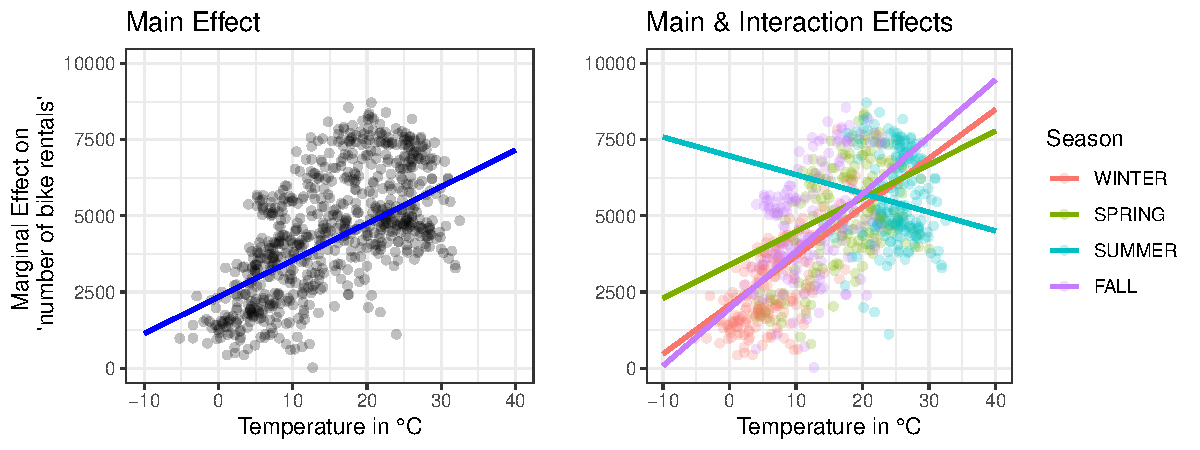
\includegraphics[width = \textwidth]{figure/lm_main_vs_interaction_effects.pdf}
\end{column}
\begin{column}{0.35\linewidth}
\begin{scriptsize}
%\begin{table}[ht]
\only<2->{\def\firstrowcolor{\rowcolor{lightgray}}}
\only<3>{\def\secondrowcolor{\rowcolor{lightgray}}}
\only<4>{\def\thirdrowcolor{\rowcolor{lightgray}}}
\only<5>{\def\fourthrowcolor{\rowcolor{lightgray}}}
\centering
\begin{tabular}{rr}
  \hline
 & Weights \\ 
  \hline
(Intercept) & 3453.9 \\ 
  seasonSPRING & 1317.0 \\ 
  seasonSUMMER & 4894.1 \\ 
  seasonFALL & -114.2 \\ 
  \firstrowcolor temp & 160.5 \\ 
  hum & -37.6 \\ 
  windspeed & -61.9 \\ 
  days\_since\_2011 & 4.9 \\
  \hline
  \secondrowcolor seasonSPRING:temp & -50.7 \\ 
  \thirdrowcolor seasonSUMMER:temp & -222.0 \\ 
  \fourthrowcolor seasonFALL:temp & 27.2 \\ 
   \hline
\end{tabular}
%\end{table}
\end{scriptsize}
\end{column}
\end{columns}
\vfill
\pause
\begin{columns}[T, totalwidth=\textwidth]
\begin{column}{0.65\linewidth}
\textbf{Interpretation}: If \code{temp} increases by 1 $^{\circ}$C, \\bike rentals
\begin{itemize}[<+->]
    \item increase by 160.5 in \code{WINTER} (reference)
    \item increase by 109.8 (= 160.5 - 50.7) in \code{SPRING}
    \item decrease by -61.5 (= 160.5 - 222) in \code{SUMMER}
    \item increase by 187.7 (= 160.5 + 27.2) in \code{FALL}
\end{itemize} %\\\vspace*{0.2cm}
\end{column}
\begin{column}{0.35\linewidth}
% \lz
% \only<6>{\textbf{Note:}
% Temperature values (on x-axis) depend on \code{season}\\
% $\leadsto$ not acknowledged by LM\\
% $\leadsto$ misleading interpretation due to extrapolation in regions with few points (e.g. low \code{temp} in \code{SUMMER})
% }
\end{column}
\end{columns}
%Value ranges of temperature differ depending on the season $\leadsto$ not acknowledged by LM
\end{frame}


\begin{frame}{Example: Quadratic Effect}
\textbf{Ex.}: Adding quadratic effect for \code{temp} \only<2>{(left) and interaction with \code{season} (right)}
\begin{columns}[T, totalwidth=\textwidth]
\begin{column}{0.7\textwidth}
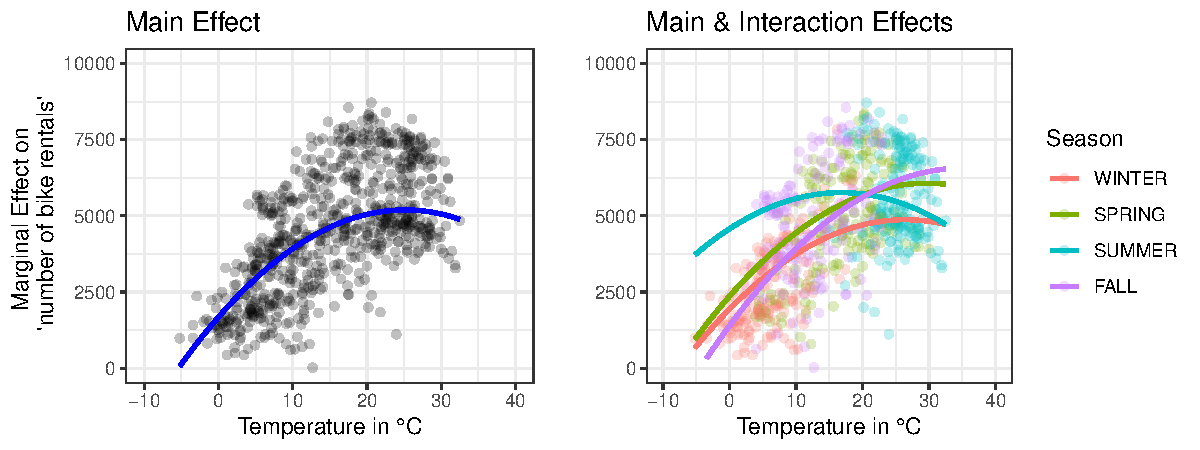
\includegraphics[width=0.5\textwidth, trim=0cm 0.1cm 10.4cm 0cm, clip]{figure/poly_main_vs_interaction_effects.pdf}\invisible<1>{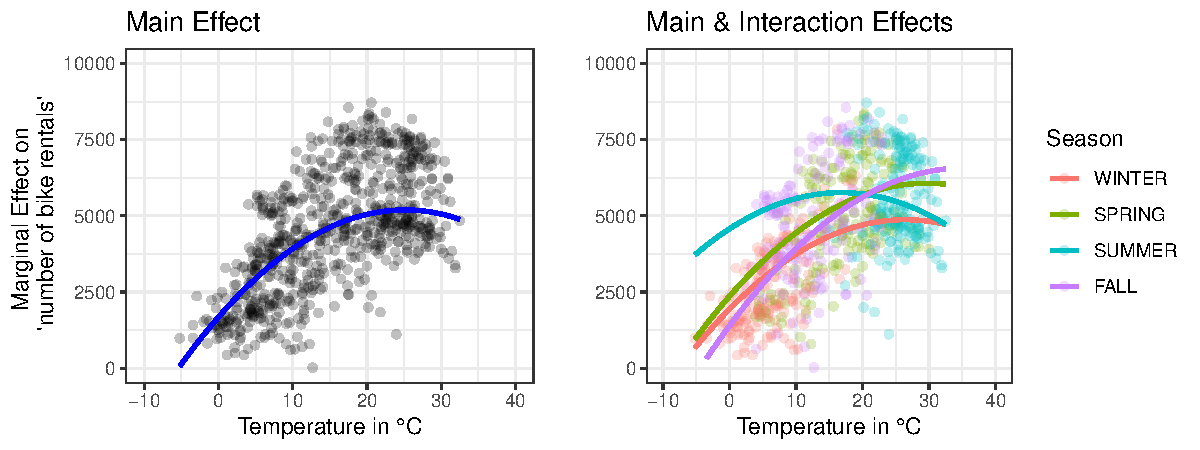
\includegraphics[width=0.5\textwidth, trim=10cm 0.1cm 0.4cm 0cm, clip]{figure/poly_main_vs_interaction_effects.pdf}}
%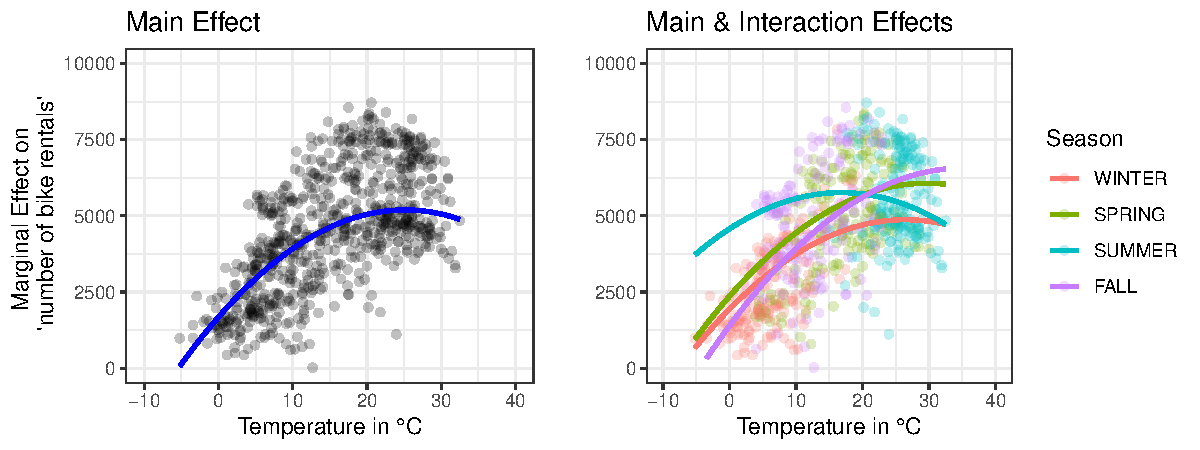
\includegraphics[width = \textwidth]{figure/poly_main_vs_interaction_effects.pdf}
%\begin{columns}[totalwidth=\textwidth]
%\begin{center}
%\adjincludegraphics[width=\textwidth, trim={0 0 {.55\width} 0}, clip]{figure/poly_main_vs_interaction_effects.pdf}

\textbf{Interpretation}: Not linear anymore!
\begin{itemize}
    \only<1>{\item \code{temp} depends on two weights: $ 280.2 \cdot x_{temp} -  5.6 \cdot x_{temp}^2$}
    \item<2> \code{temp} depends on multiple weights due to \code{season}:\\
    $\leadsto$ \code{WINTER}: \\${\color{winter}39.1} \cdot x_{temp} + {\color{winter}8.6} \cdot x_{temp}^2$ \\
    $\leadsto$ \code{SPRING}:\\ 
    $({\color{winter}39.1} {\color{spring}+407.4}) \cdot x_{temp} + ({\color{winter}8.6} {\color{spring} - 18.7}) \cdot x_{temp}^2$ \\
    $\leadsto$ \code{SUMMER}:\\ $({\color{winter}39.1}  {\color{summer}+801.1}) \cdot x_{temp} + ({\color{winter}8.6} {\color{summer} - 27.2}) \cdot x_{temp}^2$  \\
    $\leadsto$ \code{FALL}: \\$({\color{winter}39.1}  {\color{fall}+217.4}) \cdot x_{temp} + ({\color{winter}8.6} {\color{fall} - 11.3}) \cdot x_{temp}^2$ 
    % \item<2>[$\leadsto$] High-order and interaction effects make the model more flexible but also less interpretable (more weights)
    % \item<2>[$\leadsto$] High-order and interaction effects need to be specified manually (inconvenient) - ML models do this automatically
\end{itemize}

\end{column}
\begin{column}{0.3\textwidth}
%\hfill
\begin{scriptsize}
% \begin{table}[ht]
% %\centering

\def\firstrowcolor{\rowcolor{lightgray}}%
\def\secondrowcolor{\rowcolor{spring}}%
\def\thirdrowcolor{\rowcolor{summer}}%
\def\fourthrowcolor{\rowcolor{fall}}%

\only<1>{%
%\addtolength{\tabcolsep}{-1pt}
\begin{tabular}{rr}
  \hline
 & Weights \\ 
  \hline
(Intercept) & 3094.1 \\ 
  seasonSPRING & 619.2 \\ 
  seasonSUMMER & 284.6 \\ 
  seasonFALL & 123.1 \\ 
  hum & -36.4 \\ 
  windspeed & -65.7 \\ 
  days\_since\_2011 & 4.7 \\ 
  \firstrowcolor temp & 280.2 \\ 
  \firstrowcolor temp$^2$ & -5.6 \\ 
  \hline
\end{tabular}%
%\addtolength{\tabcolsep}{1pt}
}
% \end{table}
\only<2>{%
\def\firstrowcolor{\rowcolor{winter}}%
\addtolength{\tabcolsep}{-3pt}%
\begin{tabular}{rr}
  \hline
 & Weights \\ 
  \hline
(Intercept) & 3802.1 \\ 
  seasonSPRING & -1345.1 \\ 
  seasonSUMMER & -6006.3 \\ 
  seasonFALL & -681.4 \\ 
  hum & -38.9 \\ 
  windspeed & -64.1 \\ 
  days\_since\_2011 & 4.8 \\ 
 \firstrowcolor temp & 39.1 \\ 
 \firstrowcolor temp$^2$ & 8.6 \\ 
  \hline
  \hline
  \secondrowcolor seasonSPRING:temp & 407.4 \\ 
 \secondrowcolor seasonSPRING:temp$^2$ & -18.7 \\ 
  \thirdrowcolor seasonSUMMER:temp & 801.1 \\ 
 \thirdrowcolor seasonSUMMER:temp$^2$ & -27.2 \\ 
  \fourthrowcolor seasonFALL:temp & 217.4 \\ 
 \fourthrowcolor seasonFALL:temp$^2$ & -11.3 \\ 
   \hline
\end{tabular}%
\addtolength{\tabcolsep}{3pt}
}%
%Table: Weights for main effect model
\end{scriptsize}
%\end{center}
\end{column}
\end{columns}
\end{frame}


\begin{frame}{Regularization via LASSO \furtherreading{TIBSHIRANI1996}}
% \begin{itemize}
%     \item LASSO adds an $L_1$-norm penalization term ($\lambda||\theta||_1$) to the least squares optimization problem%\\
%     % $\leadsto$ Shrinks some feature weights to zero (feature selection)\\
%     % $\leadsto$ Sparser models (with fewer features) are more interpretable
%     % %Aim: Feature selection (sparsity) and regularization of feature weights
%     % \item Penalization parameter $\lambda$ must be chosen (e.g., by CV) %or depending on the number of features to keep
% \end{itemize}

\begin{columns}[T, totalwidth=\textwidth]
\begin{column}{0.6\textwidth}
\begin{itemize}
    \item LASSO adds an $L_1$-norm penalization term ($\lambda||\theta||_1$) to least squares optimization problem
    \begin{itemize}
        \item[$\leadsto$] Shrinks some feature weights to zero\\ (feature selection)
        \item[$\leadsto$] Sparser models (fewer features): \\ more interpretable
    \end{itemize}
    %Aim: Feature selection (sparsity) and regularization of feature weights
    \item Penalization parameter $\lambda$ must be chosen (e.g., by CV) %or depending on the number of features to keep
\end{itemize}
\vspace{0.2cm}
$$
min_{\theta} \bigg(\underbrace{\frac{1}{n} \sum_{i=1}^{n} (y^{(i)} - {\xi}^{\top} \theta)^2}_\text{Least square estimate for LM} + \lambda||\theta||_1\bigg) 
$$
\end{column}
\begin{column}{0.4\textwidth}
\centerline{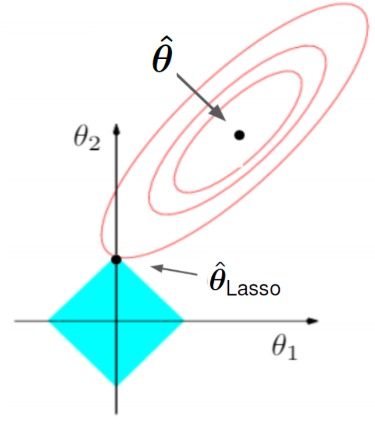
\includegraphics[width=.8\textwidth]{figure/l1_hat.png}} 
\centerline{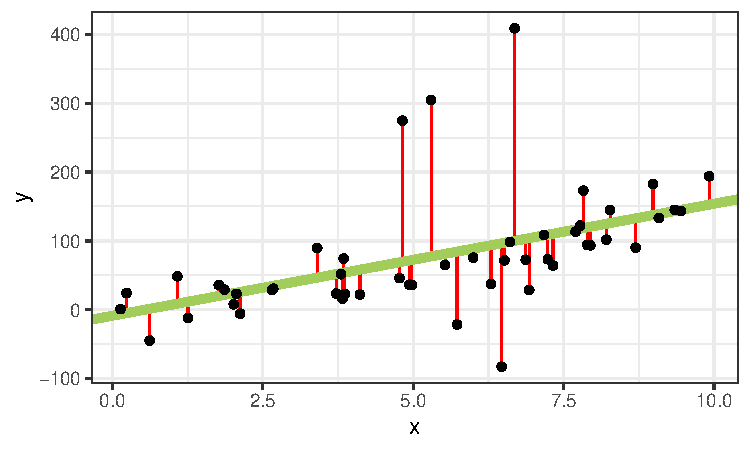
\includegraphics[width=.8\textwidth]{figure/lm_example}} 
\end{column}
\end{columns}

\end{frame}


\begin{frame}{Regularization via LASSO \furtherreading{TIBSHIRANI1996}}
\textbf{Example} (interpretation of weights analogous to LM):

\begin{itemize}
    \item LASSO with main effects and interaction \code{temp} with \code{season}
\end{itemize}
\vspace{-0.5\topsep}
\begin{columns}[c, totalwidth=\textwidth]
\begin{column}{0.65\textwidth}
\begin{itemize}
    %\item LASSO with main effects and interaction \code{temp} with \code{season}
    \item $\lambda$ is chosen $\leadsto$ 6 selected features ($\neq 0$)
    \item LASSO shrinks weights of single categories separately (due to dummy encoding)\\
    %only weights of single categories are set to zero (due to dummy encoding) not the whole feature\\
    $\leadsto$ No feature selection of whole categorical features (only w.r.t. category levels)\\
    %May be problematic for categorical features as only weights of single categories are set to zero (due to dummy encoding) instead of the whole categorical feature\\ %, polynomials and interactions
    $\leadsto$ Solution: group LASSO \furtherreading{YUANLIN2006}
\end{itemize}
\smallskip
\centering
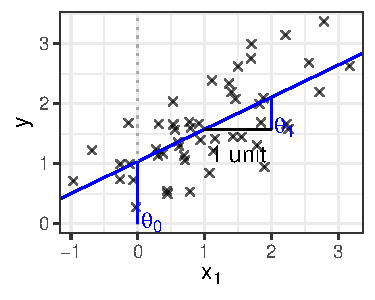
\includegraphics[width = 0.6\textwidth]{figure/reg_lm_plot_interpreted.pdf}

\end{column}
\begin{column}{0.35\textwidth}

\scriptsize
\centering
\begin{tabular}{rr}
  \hline
 & Weights \\ 
  \hline
(Intercept) & 3135.2 \\ 
  seasonSPRING & 767.4 \\ 
  seasonSUMMER & 0.0 \\ 
  seasonFALL & 0.0 \\ 
  temp & 116.7 \\ 
  hum & -28.9 \\ 
  windspeed & -50.5 \\ 
  days\_since\_2011 & 4.8 \\ 
  \hline
  seasonSPRING:temp & 0.0 \\ 
  seasonSUMMER:temp & 0.0 \\ 
  seasonFALL:temp & 30.2 \\ 
   \hline
\end{tabular}
%\end{table}
% \begin{table}[ht]
% \centering
% \begin{tabular}{rr}
%   \hline
%  & Weights \\ 
%   \hline
% (Intercept) & 2665.50 \\ 
%   seasonSPRING & 489.34 \\ 
%   seasonSUMMER & 0.00 \\ 
%   seasonFALL & 0.00 \\ 
%   hum & -19.44 \\ 
%   windspeed & -35.54 \\ 
%   days\_since\_2011 & 4.71 \\ 
%   poly(temp, 2)1 & 109.25 \\ 
%   poly(temp, 2)2 & 0.00 \\ 
%   \hline
% \end{tabular}
% \end{table}
\end{column}
\end{columns}


%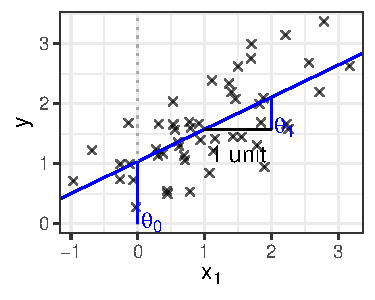
\includegraphics[width = 0.8\textwidth]{figure/reg_lm_plot_interpreted.pdf}


\end{frame}
\endlecture

\end{document}
